The $32^3$ run is the first test of the chain (particle mass $2.1\times10^{13}$\,\Msunh{}, at most 15 halos per
snapshot). Table~\ref{tab:p32} and the grey lines of Fig.~\ref{fig:pvz} summarise the particle comparison.

\begin{table}[H]
\centering\small
\begin{tabular}{@{}rrcccccccc@{}}
\toprule
out & $z$ & corr$(\phi)$ & $\frac{{\rm rms}\,\Delta\phi}{{\rm rms}\,\phi}$ & FFT$_{x}$ & offset & med $|\Delta x|$ & 90\% $|\Delta x|$ & med $|\Delta v|$ & corr$(v)$ \\
 & & & & & \kms & \Mpch & \Mpch & km\,s$^{-1}$ & \\
\midrule
0 & 11.98 & 0.99965 & 0.026 & 0.082 & $+1392$ & 0.016 & 0.029 & 6.3 & 0.9989 \\
19 & 2.96 & 0.99972 & 0.024 & 0.103 & $+451$ & 0.098 & 0.167 & 13.3 & 0.9980 \\
46 & 1.00 & 0.99520 & 0.098 & 0.117 & $+308$ & 0.205 & 0.364 & 17.9 & 0.9633 \\
64 & 0.50 & 0.98510 & 0.173 & 0.147 & $-419$ & 0.271 & 0.531 & 20.8 & 0.9123 \\
100 & 0.00 & 0.96891 & 0.253 & 0.220 & $-2011$ & 0.379 & 0.891 & 24.9 & 0.8151 \\
\bottomrule
\end{tabular}
\caption{$32^3$, particle by particle. FFT$_x$: rms difference of the FFT potentials computed from the two codes'
particle positions, over rms $\phi$. Offset: median $\phi_{\rm pkd} - \phi_{\rm Gadget}$ after removing \pkd{}'s
self-term ($-1.9\times10^7$ at $z=12$, $-1.4\times10^6$\,\kms{} at $z=0$).}
\label{tab:p32}
\end{table}

\begin{itemize}
\item \textbf{Potential.} Until $z\approx3$ the two potentials agree to 2--3\% rms (correlation 0.9997). Afterwards the
difference grows to 25\% at $z=0$; the FFT potentials of the two codes' own particle positions differ by
22\%, so most of the late-time difference comes from the particles being in different places, not from
the force solvers. The zero points agree to $\lesssim 2\times10^3$\,\kms{} (0.1\% of the self-term that \pkd{} carries).
\item \textbf{Positions and velocities.} The median particle separation grows from 16\,$h^{-1}$kpc at $z=12$ to
0.38\,\Mpch{} at $z = 0$ ($1.8\,\epsilon_G$, 6\% of the mean interparticle spacing 6.25\,\Mpch{}), the median
velocity difference from 6 to 25\,km\,s$^{-1}$. The rms velocity difference (314\,km\,s$^{-1}$ at $z=0$) is
dominated by particles in halos, where trajectories are chaotic: there the median is small but the tail long
(Fig.~\ref{fig:p32}). The rms velocities of the two runs differ by 0.4\% at $z = 12$ and 1.7\% at $z = 0$.
\item \textbf{Halos.} Rockstar finds 13 host halos in \gad{} and 8 in \pkd{} at $z=0$; 4 are matched one to one
(the others merge or split differently at the 30--40 particle limit). Matched masses agree to a few per cent.
\item \textbf{Stacked potential} (Fig.~\ref{fig:s32}). Around the 9 halos above $4\times10^{14}$\,\Msunh{} the mean
potential of the two codes agrees within the jackknife errors from 1 to 50\,\Mpch{}; inside $\sim 0.5$\,\Mpch{}
\pkd{}'s is deeper, as expected from its smaller effective softening (\pkd{}'s force becomes Newtonian at
$1.0\,\epsilon_G$, \gad{}'s at $2.8\,\epsilon_G$). With 1--9 halos per bin these numbers are indicative only.
\end{itemize}

\begin{figure}[H]
\centering
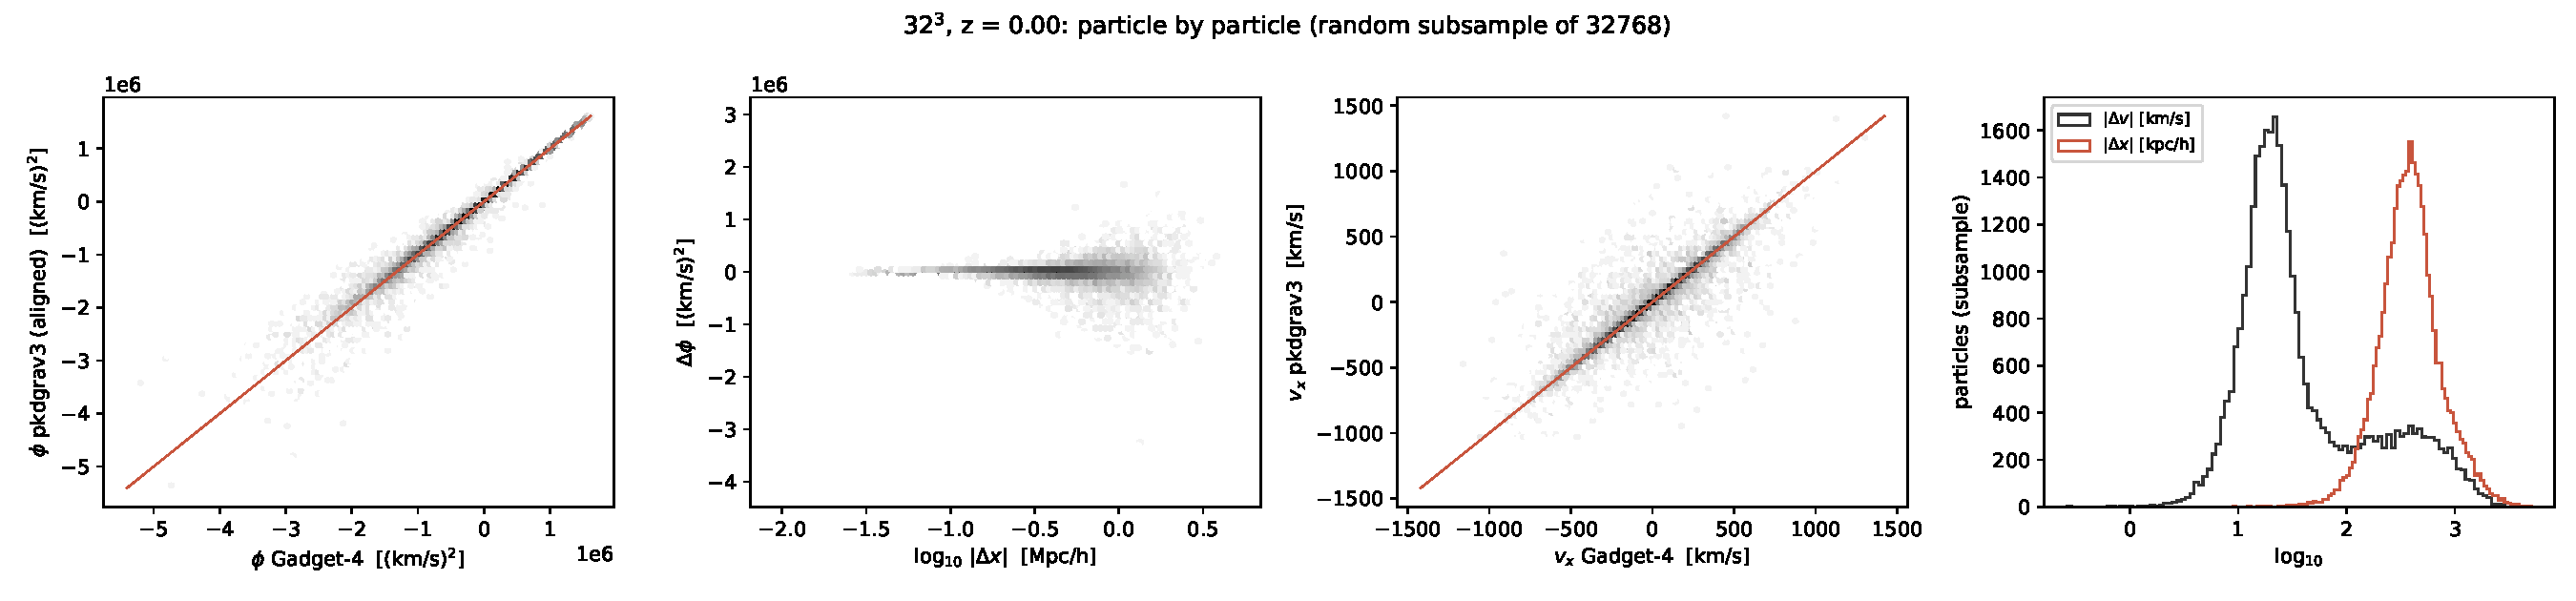
\includegraphics[width=\textwidth]{figs/particles_32_z0.pdf}
\caption{$32^3$, $z=0$, every particle: potentials (\pkd{} aligned to \gad{}'s zero point), potential difference
against particle separation, $v_x$, and the distributions of $|\Delta v|$ and $|\Delta x|$.}
\label{fig:p32}
\end{figure}

\begin{figure}[H]
\centering
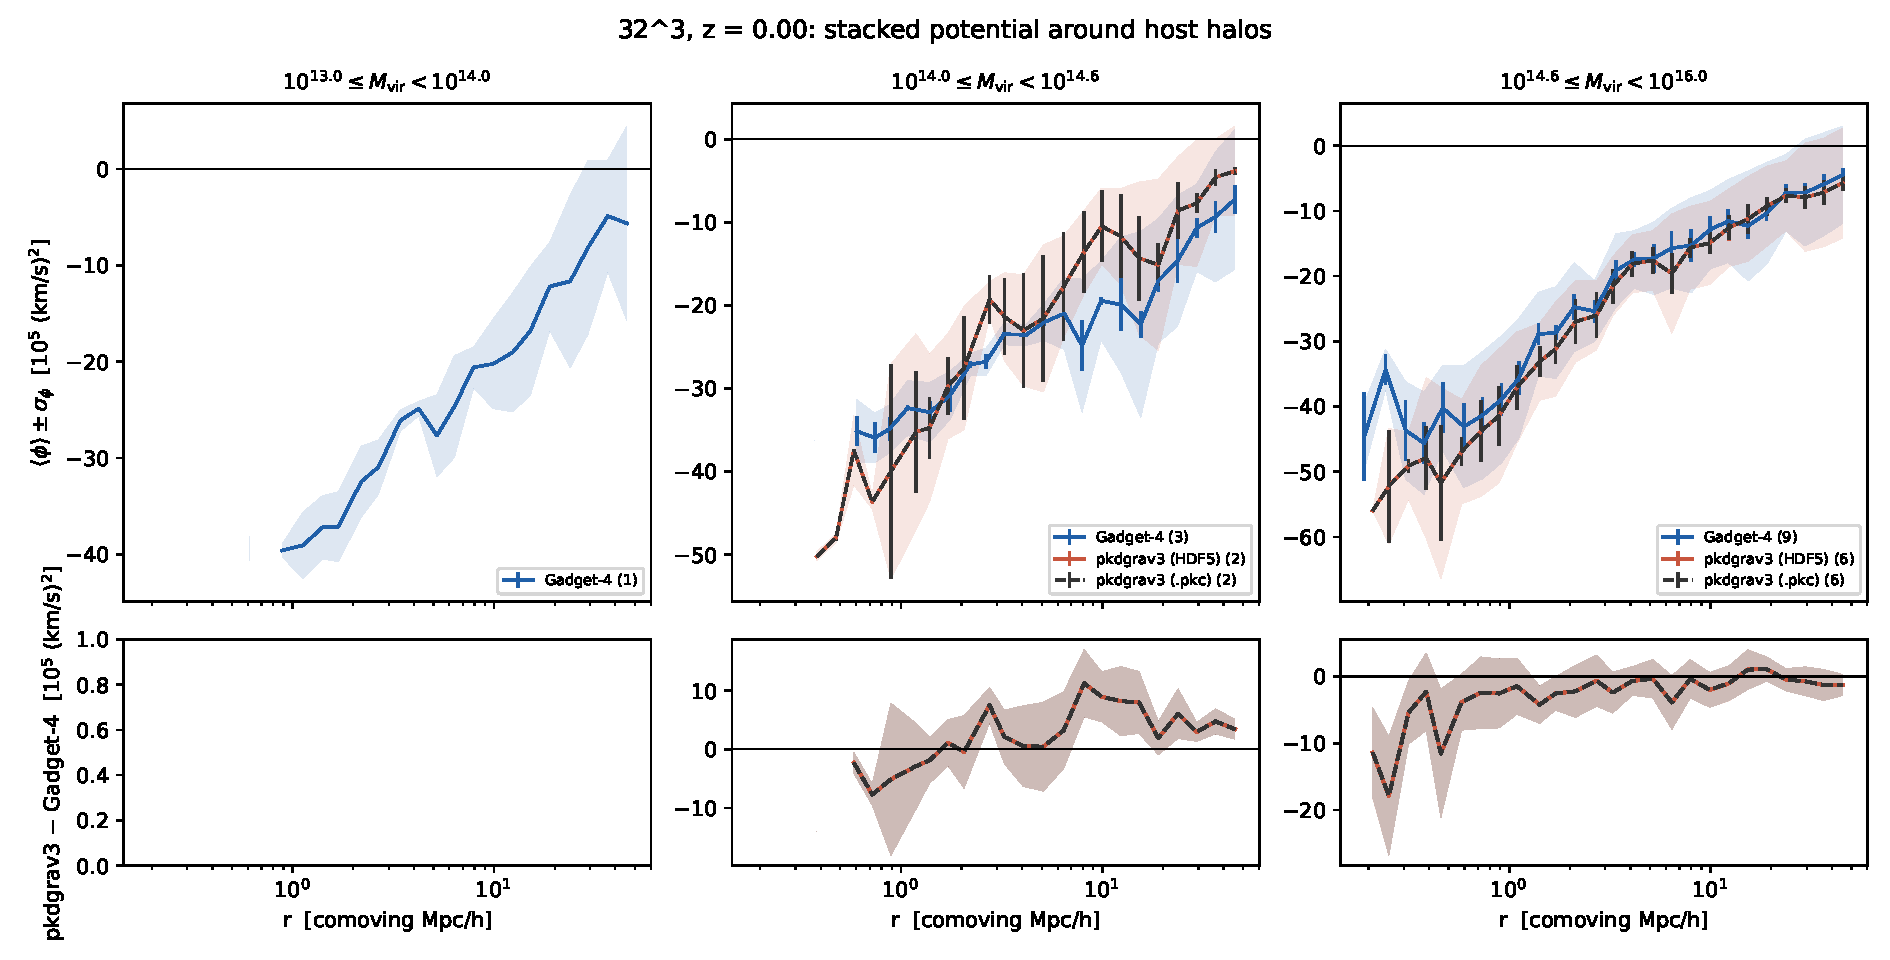
\includegraphics[width=\textwidth]{figs/stack_32_out100.pdf}
\caption{$32^3$, $z=0$: stacked potential around host halos in three $M_{\rm vir}$ bins (number of halos in the
legend). Line with error bars: mean and jackknife error; band: $\pm\sigma_\phi$, the scatter of the potential over
all pairs in the shell. Bottom: \pkd{} $-$ \gad{} (HDF5 and \texttt{.pkc} coincide).}
\label{fig:s32}
\end{figure}

The volume-weighted and linear-bin stacks were made at $32^3$ too ($64^3$ grid, spacing 3.1\,\Mpch). With 1--12
halos per bin and 0.2\,\Mpch{} shells, almost every linear shell has fewer than 50 pairs and is masked. They are in
\fp{data/pkd32_vs_gadget32_r1/profiles} and the notebook, but carry no information beyond the $256^3$ results.

\begin{figure}[H]
\centering
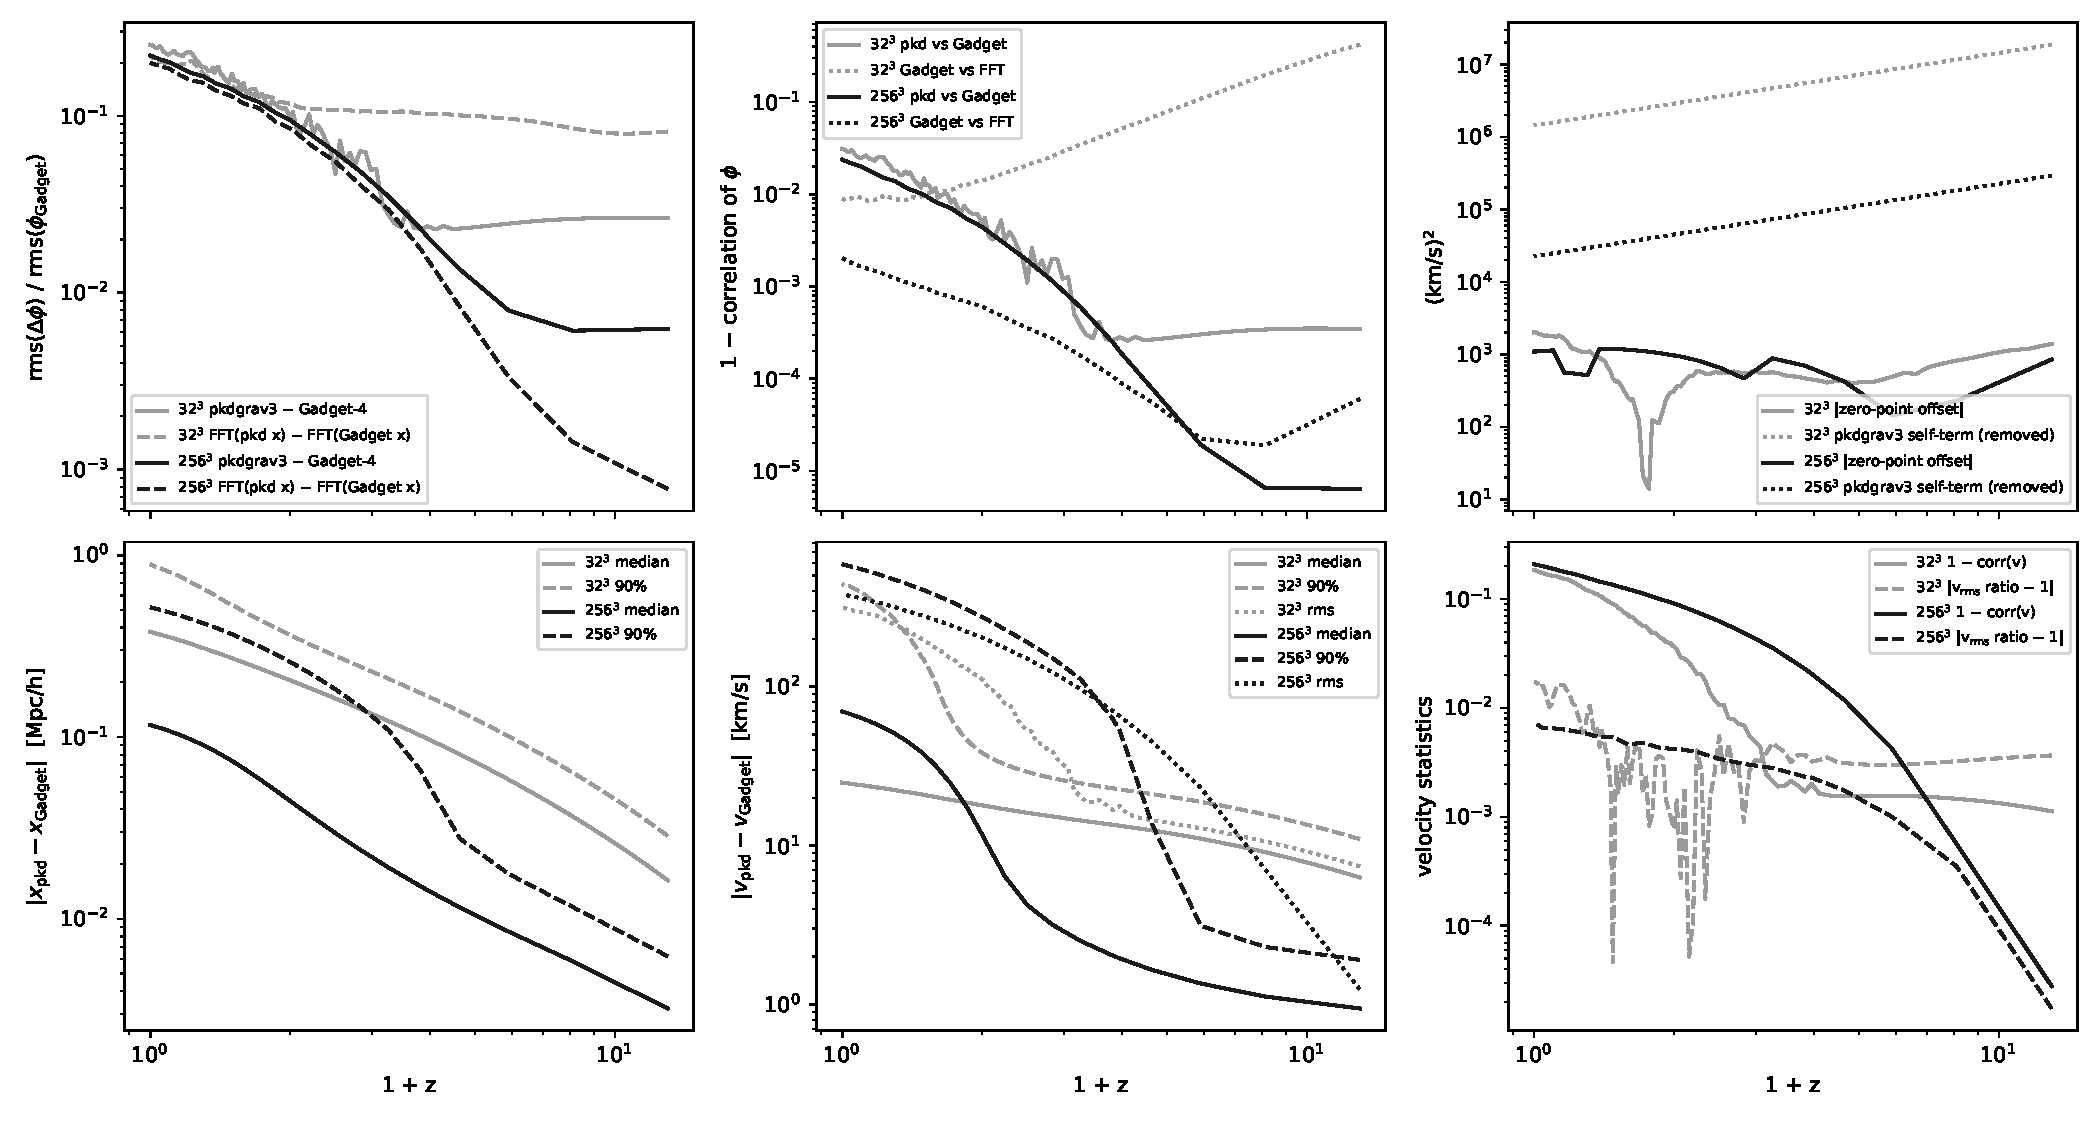
\includegraphics[width=\textwidth]{figs/particles_vs_z.pdf}
\caption{Particle-by-particle statistics against redshift (grey: $32^3$, black: $256^3$).
Top: rms potential difference over rms potential (solid) and the same for the FFT potentials of the two codes'
particle positions (dashed); $1-$correlation of the potentials; zero-point offset and \pkd{}'s removed self-term.
Bottom: particle separation, velocity difference, velocity correlation and rms-velocity ratio.}
\label{fig:pvz}
\end{figure}

\begin{figure}[H]
\centering
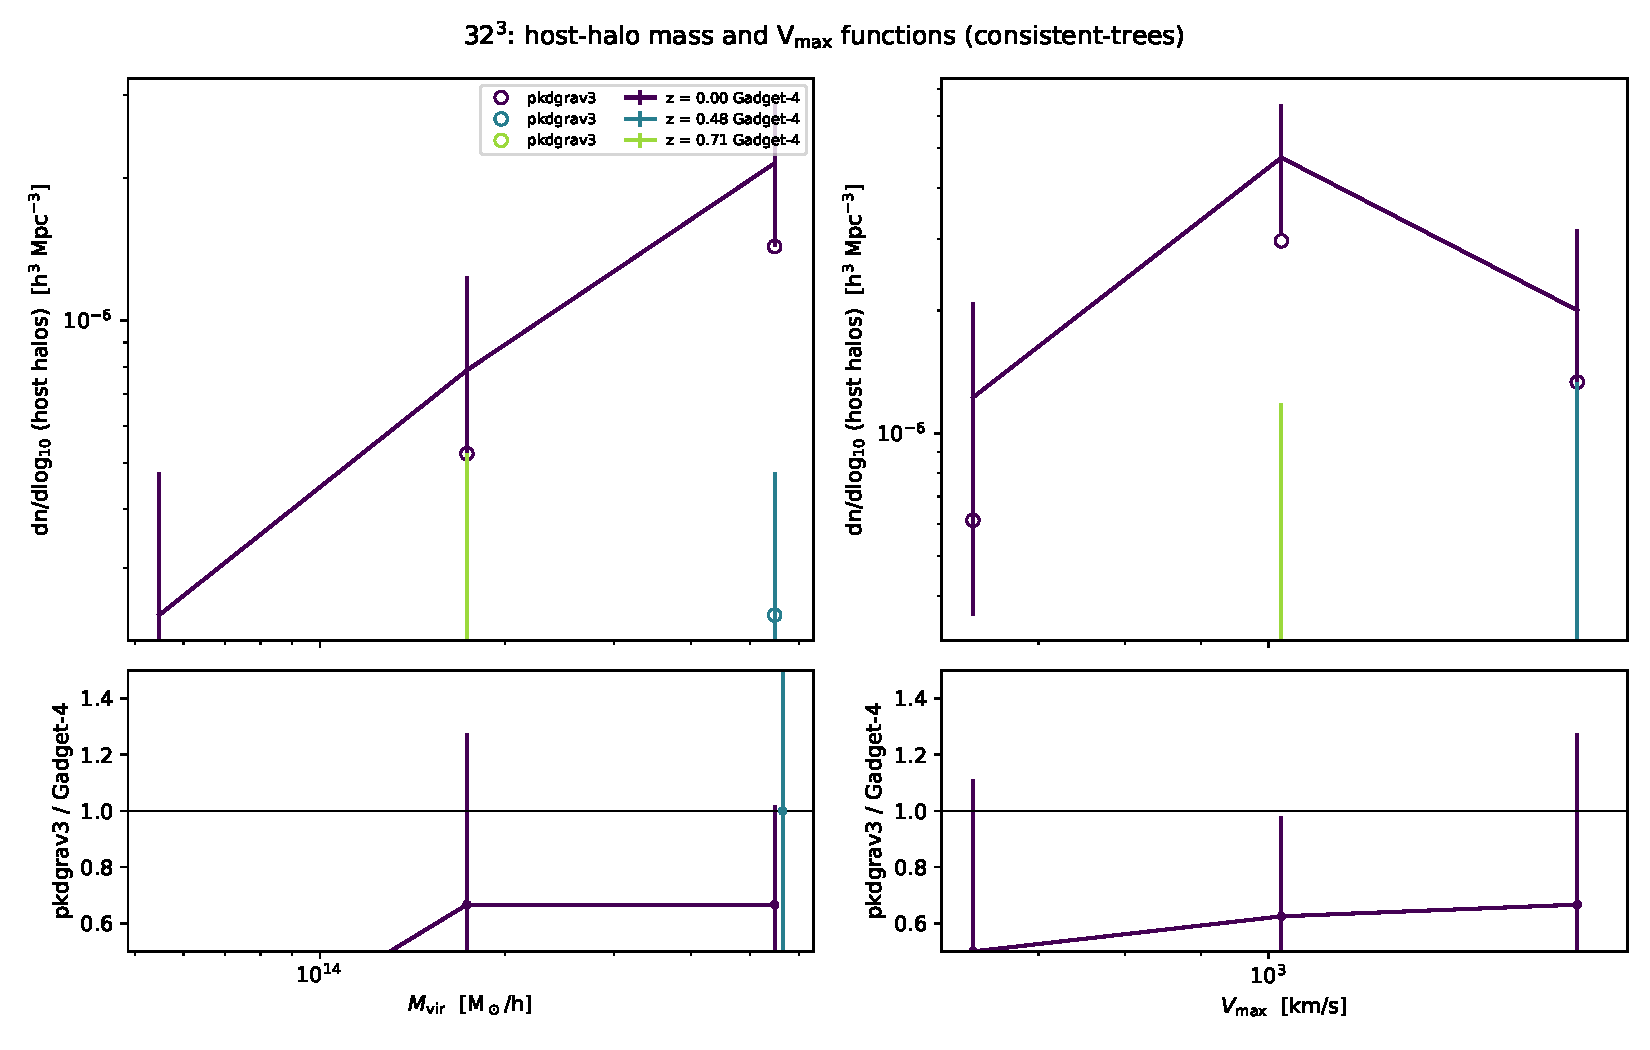
\includegraphics[width=0.75\textwidth]{figs/halo_mf_32.pdf}
\caption{$32^3$: host-halo $M_{\rm vir}$ and $V_{\max}$ functions (Rockstar) of both codes; with $\le15$ halos
per snapshot this is only a test of the tool.}
\label{fig:mf32}
\end{figure}
